% Chapter Template

\chapter{Desarrollo: Iteración II} % Main chapter title

\label{Chapter7} % Change X to a consecutive number; for referencing this chapter elsewhere, use \ref{ChapterX}

\steveCabecera{Capítulo 7. \emph{Iteración II}} % Change X to a consecutive number; this is for the header on each page - perhaps a shortened title

%----------------------------------------------------------------------------------------
%	SECTION 1
%----------------------------------------------------------------------------------------
\section{Introducción}
En este capítulo se documentan aspectos relevantes relacionados con la codificación que se realizó en la segunda iteración de desarrollo del software.\\
Se explicaran los Casos de Uso más interesantes de los contemplados para esta iteración.
Se comentará sobre el repositorio de locaciones con el que se obtendrá la información de ubicación del teléfono.
Finalmente se introducirá la metodología, conceptos y herramientas utilizadas para realizar las pruebas unitarias y pruebas de interfaz de usuario.

\section{Casos de Uso Implementados}
Para la presente iteración se implementaron los siguientes casos de uso.
\begin{enumerate}
	\item Calibrar Módulo
	\item Borrar Módulos Inaccesibles
	\item Resetear Calibración
	\item Actualizar Geolocalización
	\item Eliminar Usuario
	\item Crear Usuario
\end{enumerate}

A continuación se documentaran aquellos que presentan los escenarios más interesantes.

\subsection{Resetear Calibración}
Un usuario de nivel administrador ingresa a la pantalla de configuración de un módulo y presiona el botón 
para reiniciar la calibración de dicho módulo.
Esta operación ejecuta el RPC para modificar el atributo GATE-STATUS almacenado en el módulo y le asigna el valor UNKNOWN
de forma tal que la próxima vez que algún usuario accione dicho módulo se activará el wizard de calibración.
Este caso de uso utiliza solo un RPC y falla en dos escenarios con dos tipos de error

\begin{itemize}
	\item Error de comunicación con el módulo
	\item El usuario fue eliminado del módulo.
\end{itemize}

En el diagrama de la figura ~\ref{fig:act_resetCalib} se puede observar el flujo del algoritmo implementado para este caso de uso.
\begin{figure}[htbp]
	\centering
	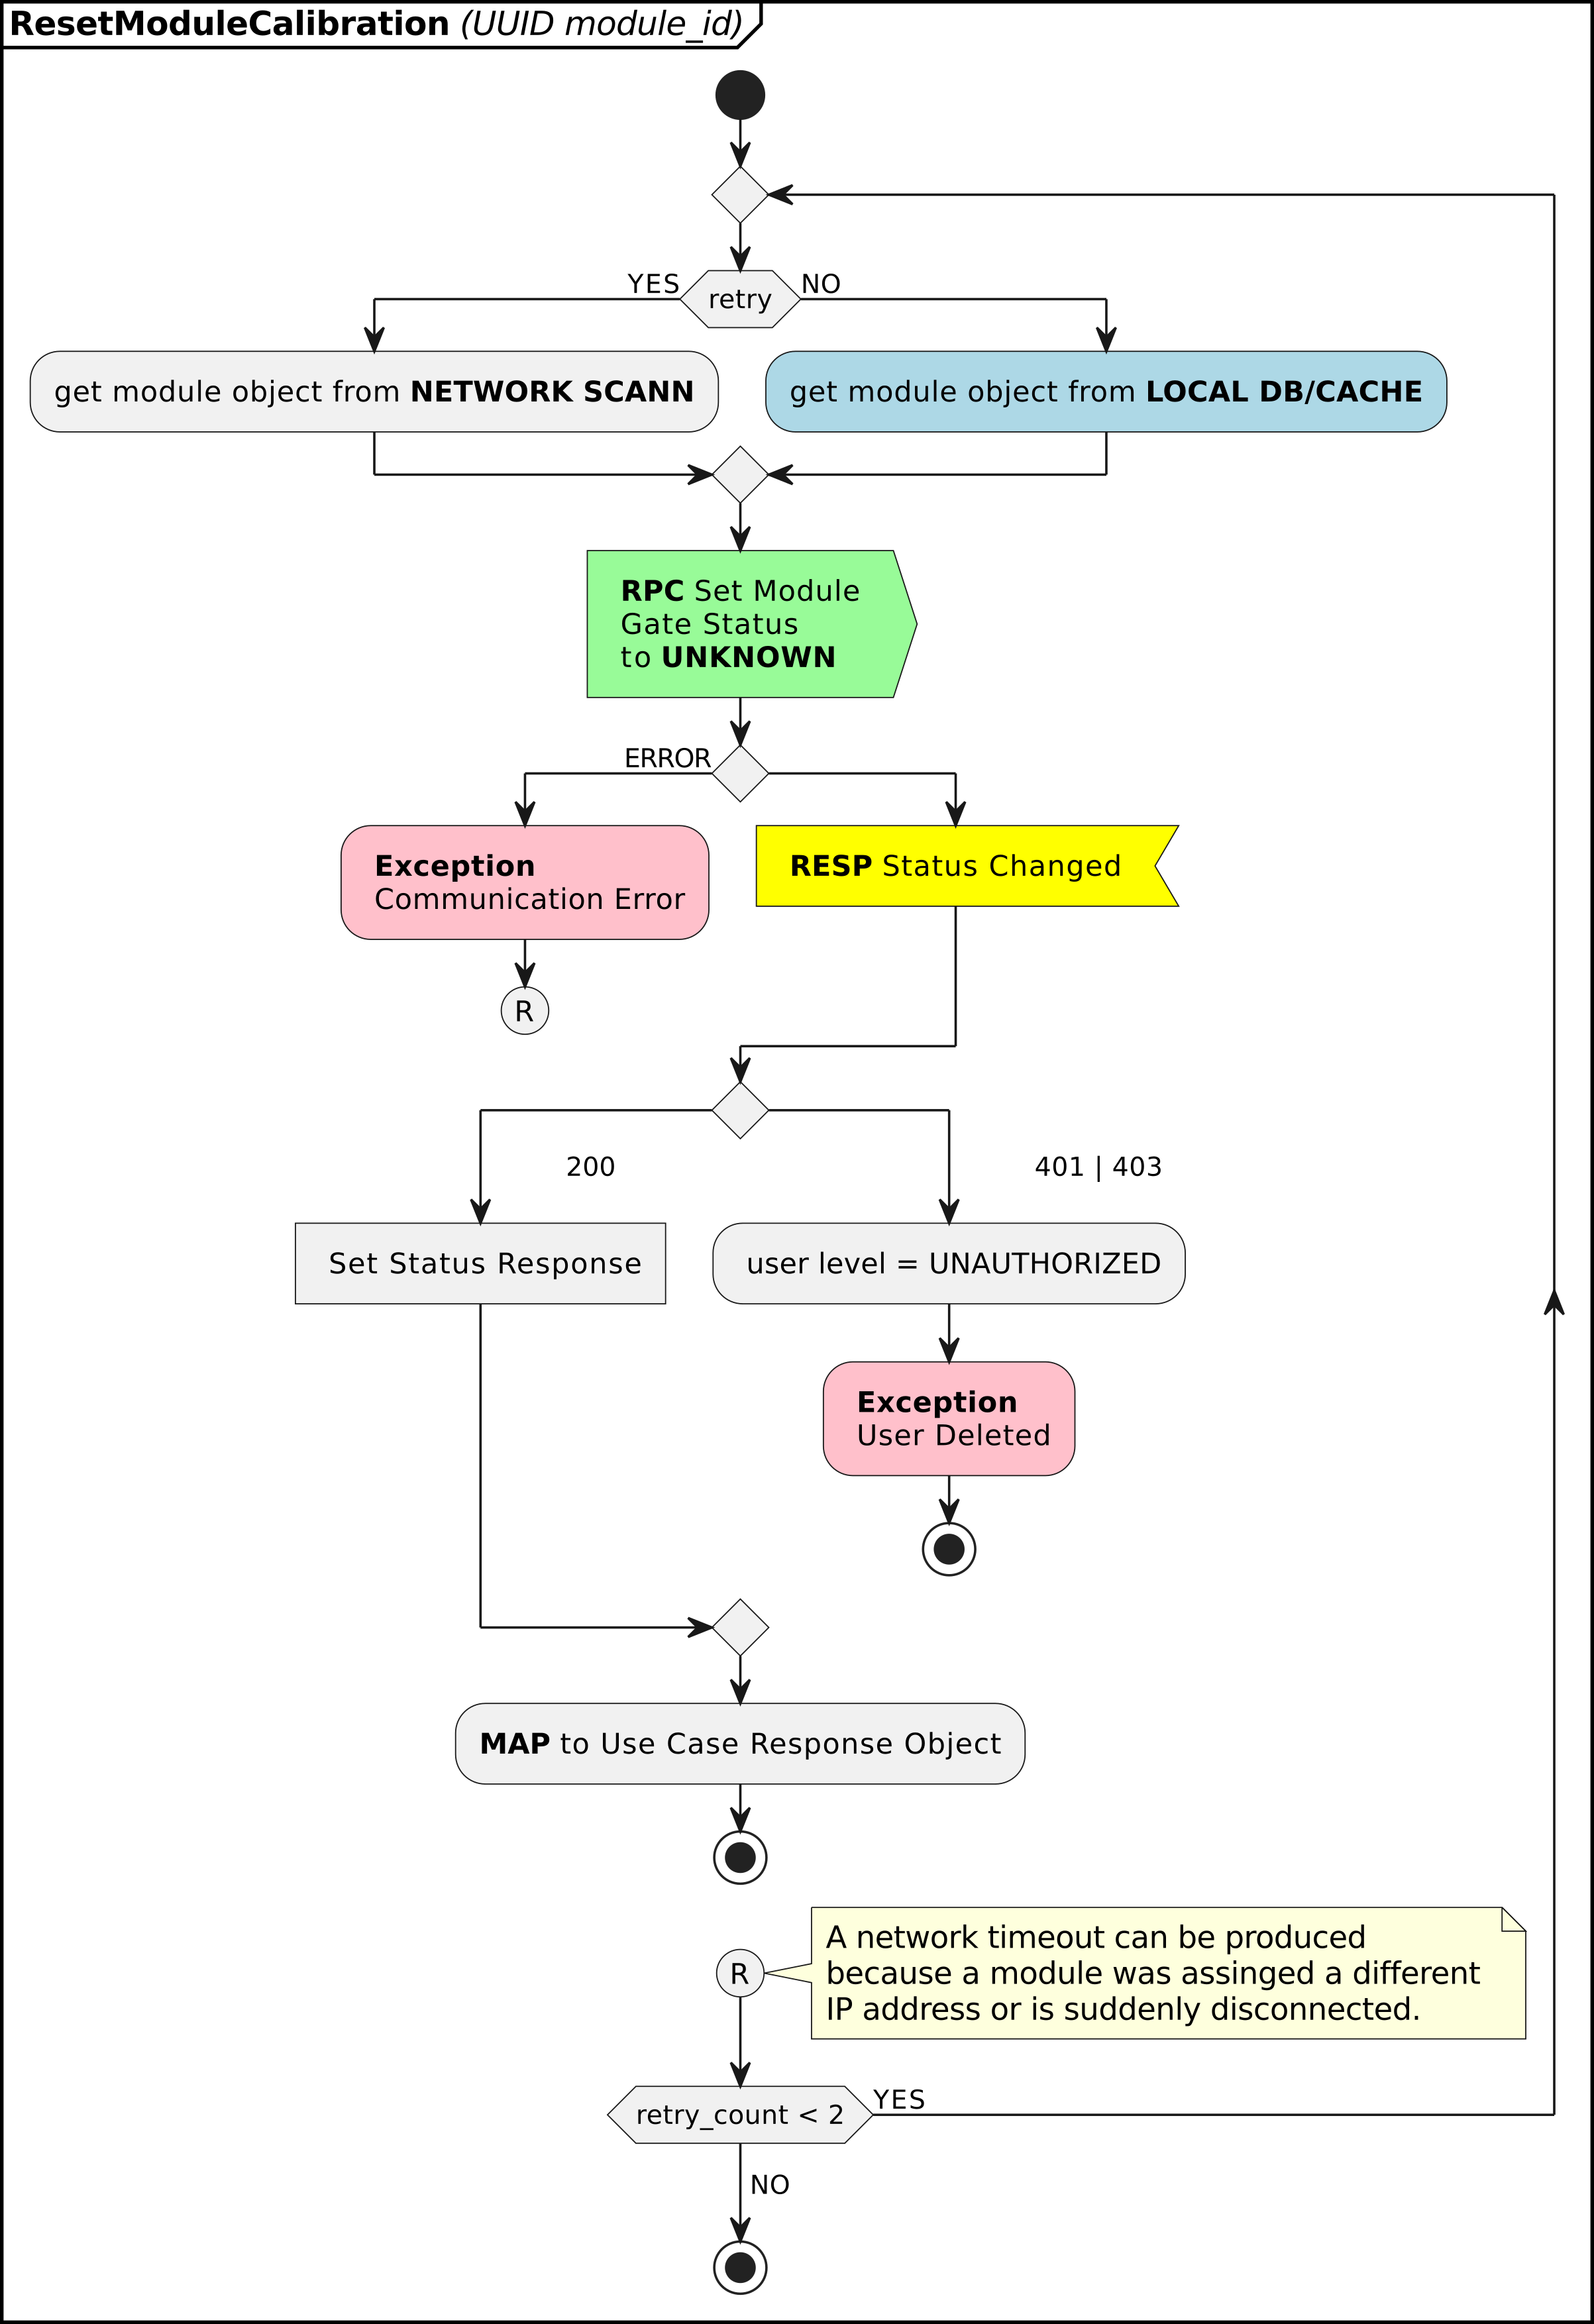
\includegraphics[width=0.8\textwidth]{Figures/iter2/ACT_resetCalib.png}
	\rule{35em}{1pt}
	\caption[Actividades Resetear Calibración]{Diagrama de actividades de la implementación del caso de uso: Resetear Calibración.}
	\label{fig:act_resetCalib}
\end{figure}

\subsection{Obtener Geolocalización}
Un usuario ingresa a la pantalla de configuración de un módulo y toca el ícono de ubicación.
Esta acción debería actualizar el texto que indica latitud, longitud y la dirección urbana que se desea asignar a dicho módulo.
Para esta operación no se ejecuta ningún RPC sino que se trata de llamadas a métodos de la librería Android-ReactiveLocation por mcharmas, que hace de interfaz reactiva con el servicio de ubicación de android.
El caso de uso puede fallar en 2 escenarios cuando los métodos no generan resultados después de realizar las consultas.
Para ambos escenarios se contempla el re-intento de hasta 3 veces ya que obtener resultados nulos es una situación frecuente.

En el diagrama de la figura ~\ref{fig:act_geoloc} se puede observar el flujo del algoritmo implementado para este caso de uso.

\begin{figure}[htbp]
	\centering
	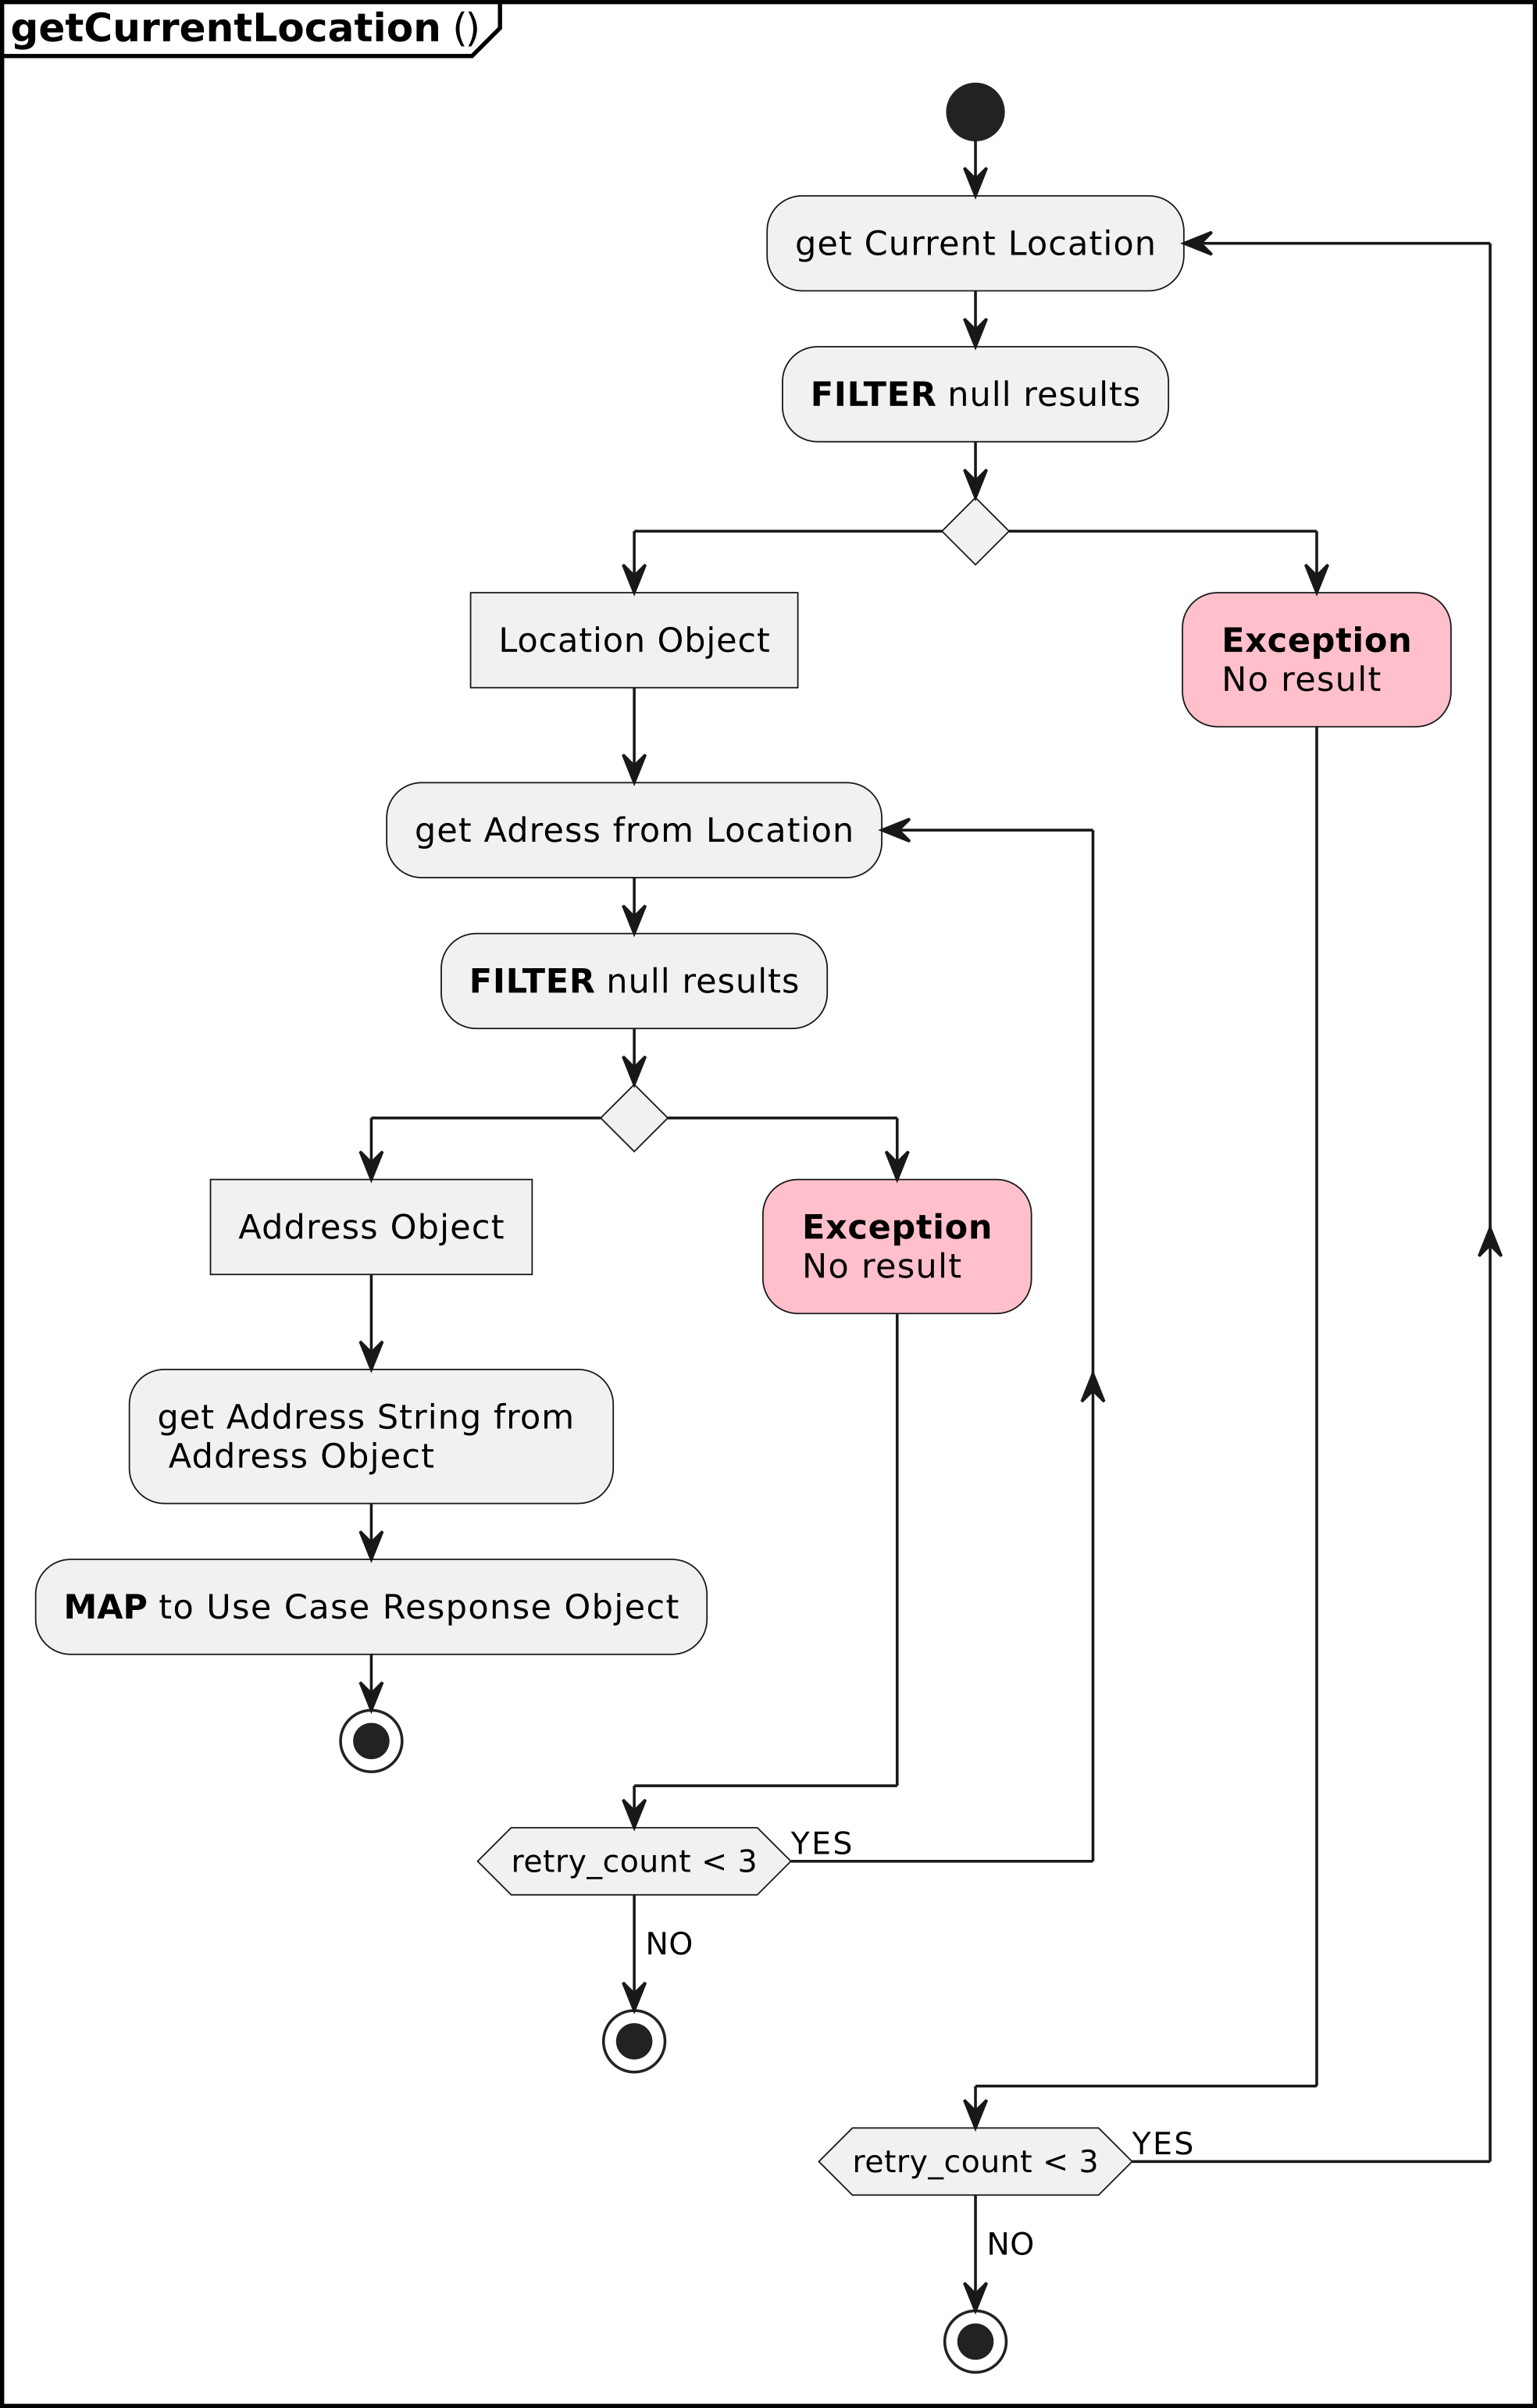
\includegraphics[width=0.7\textwidth]{Figures/iter2/ACT_geoloc.png}
	\rule{35em}{1pt}
	\caption[Actividades Obtener Geolocalización]{Diagrama de actividades de la implementación del caso de uso: Obtener Geolocalización.}
	\label{fig:act_geoloc}
\end{figure}

\subsection{Eliminar Usuario}
Un usuario administrador ingresa a la pantalla de gestión de usuarios de un módulo, sobre la lista de usuarios mantiene presionado el ícono por unos segundos para eliminar un usuario. Se muestra una barra de progreso y la acción termina mostrando un mensaje de éxito o error.
Para esta operación se emplea un único RPC y puede fallar en tres escenarios, a saber:
\begin{itemize}
	\item Error de comunicación con el módulo
	\item El usuario dejó de ser Administrador.
	\item El usuario que se intenta eliminar ya no existe.
\end{itemize}

En el diagrama de la figura ~\ref{fig:act_deleteUser} se puede observar el flujo del algoritmo implementado para este caso de uso.

\begin{figure}[htbp]
	\centering
	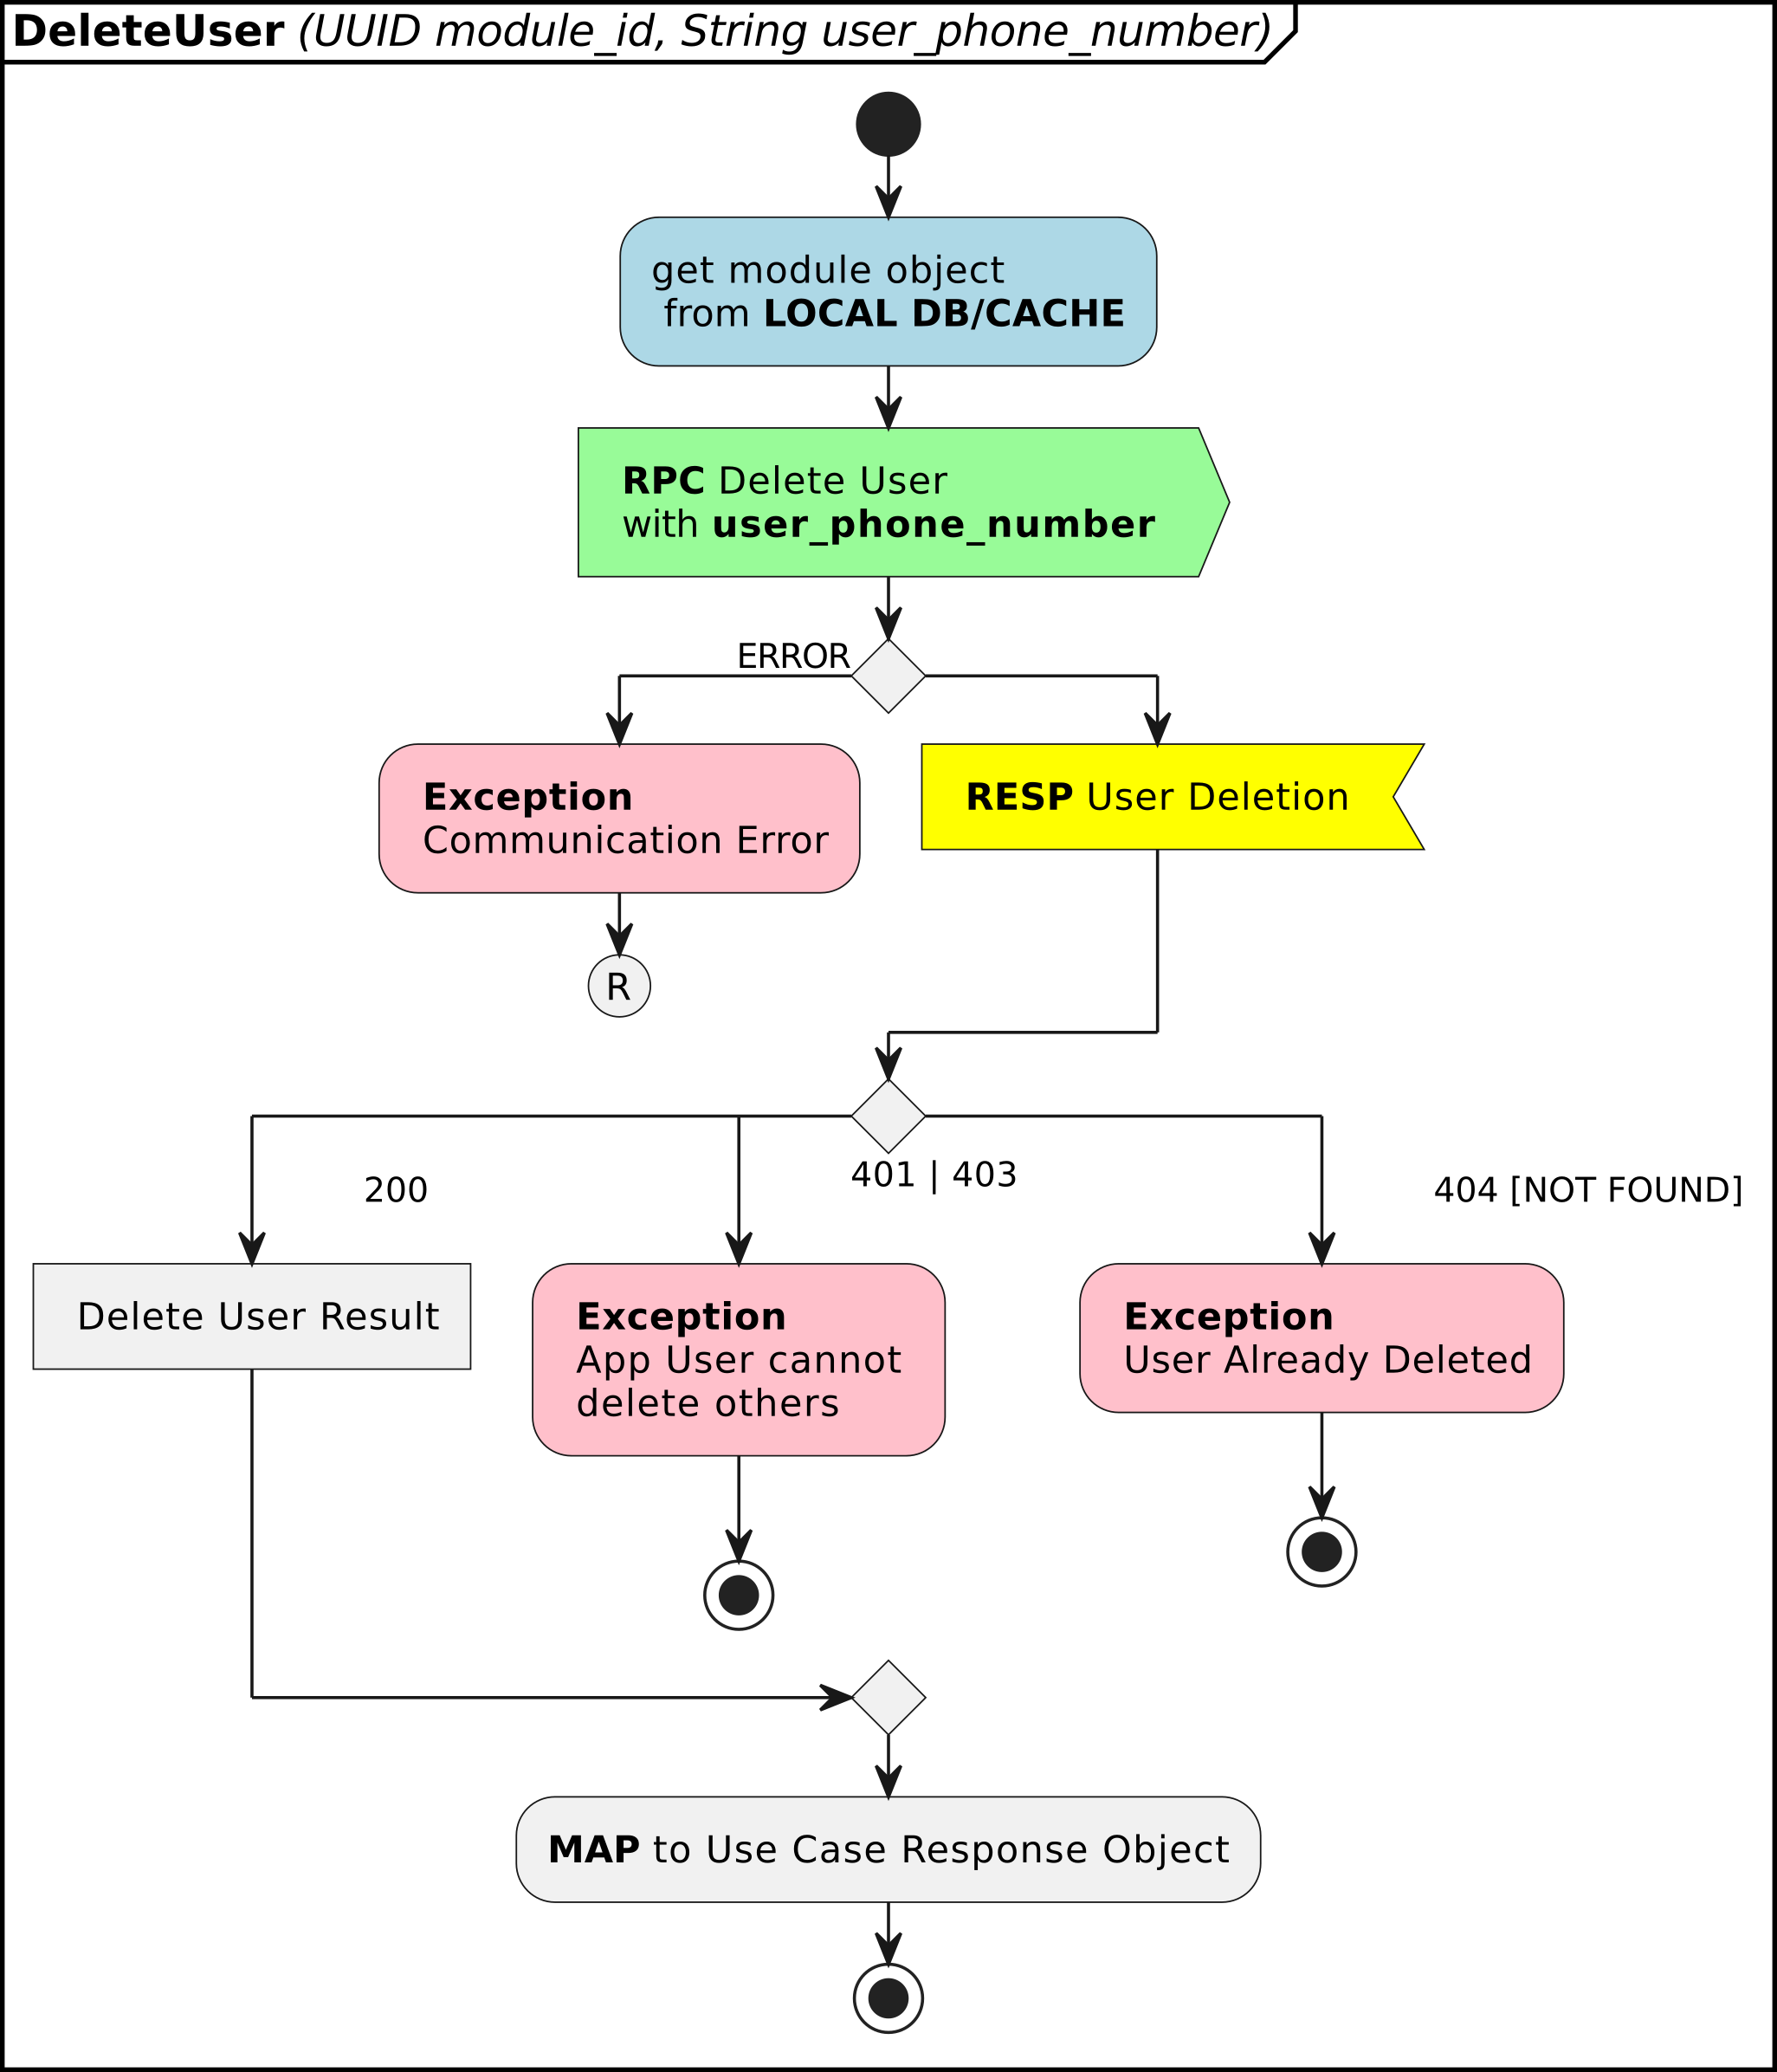
\includegraphics[width=0.7\textwidth]{Figures/iter2/ACT_deleteUser.png}
	\rule{35em}{1pt}
	\caption[Actividades Eliminar Usuario]{Diagrama de actividades de la implementación del caso de uso: Eliminar Usuario.}
	\label{fig:act_deleteUser}
\end{figure}

\section{Pruebas Automáticas}

\subsection{Dobles de Prueba}
Todo objeto o componente utilizado en las pruebas de software para reemplazar una dependencia real del sistema bajo prueba (SUT: System Under Test). Estos objetos se utilizan para aislar el SUT de sus dependencias, permitiendo un control más preciso sobre las condiciones de la prueba y facilitando la simulación de diferentes escenarios.
Existen diversos tipos de dobles de prueba caracterizados cada uno por el propósito de su empleo en cada caso, a saber:

\begin{itemize}
	\item \textbf{Mock}: Objeto ``maqueta'' que imita la interfaz del objeto dependencia real con el objetivo de simular interacciones con el SUT para dado caso de prueba.
	\item \textbf{Stub}: Trozo de código que se utiliza como sustituto funcional para implementaciones reales con el objetivo de emular precondiciones del caso de prueba.
	\item \textbf{Spy}: Hace referencia a la capacidad de un objeto de verificar la utilización de sus métodos con el propósito de evaluar la ocurrencia de las interacciones del SUT con tal objeto dependencia que determinarán si el caso de prueba pasa son éxito o resulta fallido.
	\item \textbf{Dummy}: Reemplazo de una dependencia que es necesaria para cumplir alguna firma pero que puede ser no utilizada en el caso de prueba.
	\item \textbf{Fake}: Re-Implementación funcional exclusiva de un objeto dependencia empleado por uno o todos los casos de prueba de un SUT. Se utiliza cuando el entorno de pruebas presenta limitaciones o restricciones que hacen necesaria una implementación reducida, simplificada o especializada de dicha dependencia. 
\end{itemize}

Teniendo en cuenta estas definiciones un Mock es un Stub, es un Spy y es un Dummy. 
Sin embargo un objeto Fake no tiene relación con los otros tipos ya que es una implementación independiente y funcional por si misma que será utilizada solo en el entorno de pruebas para ejecutar los casos de prueba.

Los casos de pruebas unitarias para la aplicación móvil se implementaron utilizando el framework \texttt{JUnit} y la librería \texttt{Mockito} que permite la creación de dobles de prueba de una manera simplificada facilitando su codificación.\\
Aunque \texttt{Mockito} respeta las definiciones de dobles de prueba anteriormente detalladas existe una particularidad en cuanto a la declaración de objetos tipo Spy. La declaración explícita de un Spy en \texttt{Mockito} se realiza sobre la implementación ``real'' de una dependencia agregando el wrapper que permite evaluar la utilización de sus métodos. Así mismo todos los dobles de prueba tipo Mock incorporan la capacidad de un Spy por defecto.

\subsection{RxJava Test}
La librería RXJava ofrece algunas utilidades para evaluar casos de prueba. Entre ellas podemos encontrar a un suscriptor de prueba y un scheduler de prueba.
\begin{itemize}
	\item \texttt{TestSubscriber}: Permite verificar si el stream reactivo terminó correctamente o con error. La cantidad de total de elementos emitidos y comparar el stream con una lista de elementos. 
	\item \texttt{TestScheduler}: Permite emular el paso del tiempo. 
\end{itemize}
Teniendo en cuenta que las partes más relevantes del código fueron implementadas utilizando el paradigma reactivo. Con estas herramientas a disposición es posible conseguir un mayor control sobre la validación de los casos de prueba.

\subsection{Convención de Nombrado}
Se optó por utilizar la convención de nombres para casos de prueba semejante al lenguaje Gherkin. Con esta nomenclatura es posible entender las precondiciones de la prueba (\texttt{Given}), el disparador del caso de prueba (\texttt{When}) y el resultado esperado (\texttt{Then}) con solo leer el nombre del test.
Entonces el nombre de la prueba tendrá el siguiente formato:\\
\texttt{Given\_...\_When\_...\_Then\_...\{\}}

\subsection{Metodología}
Para asegurar la total cobertura de los casos de prueba para las clases y métodos más relevantes se dibujaron los diagramas de actividades correspondientes y se identificaron las ramas condicionales que definen los escenarios de ejecución. Se determina así la complejidad ciclomática y con ello el número total de casos de prueba necesarios para cubrir todos los escenarios.

\begin{figure}[htbp]
	\centering
	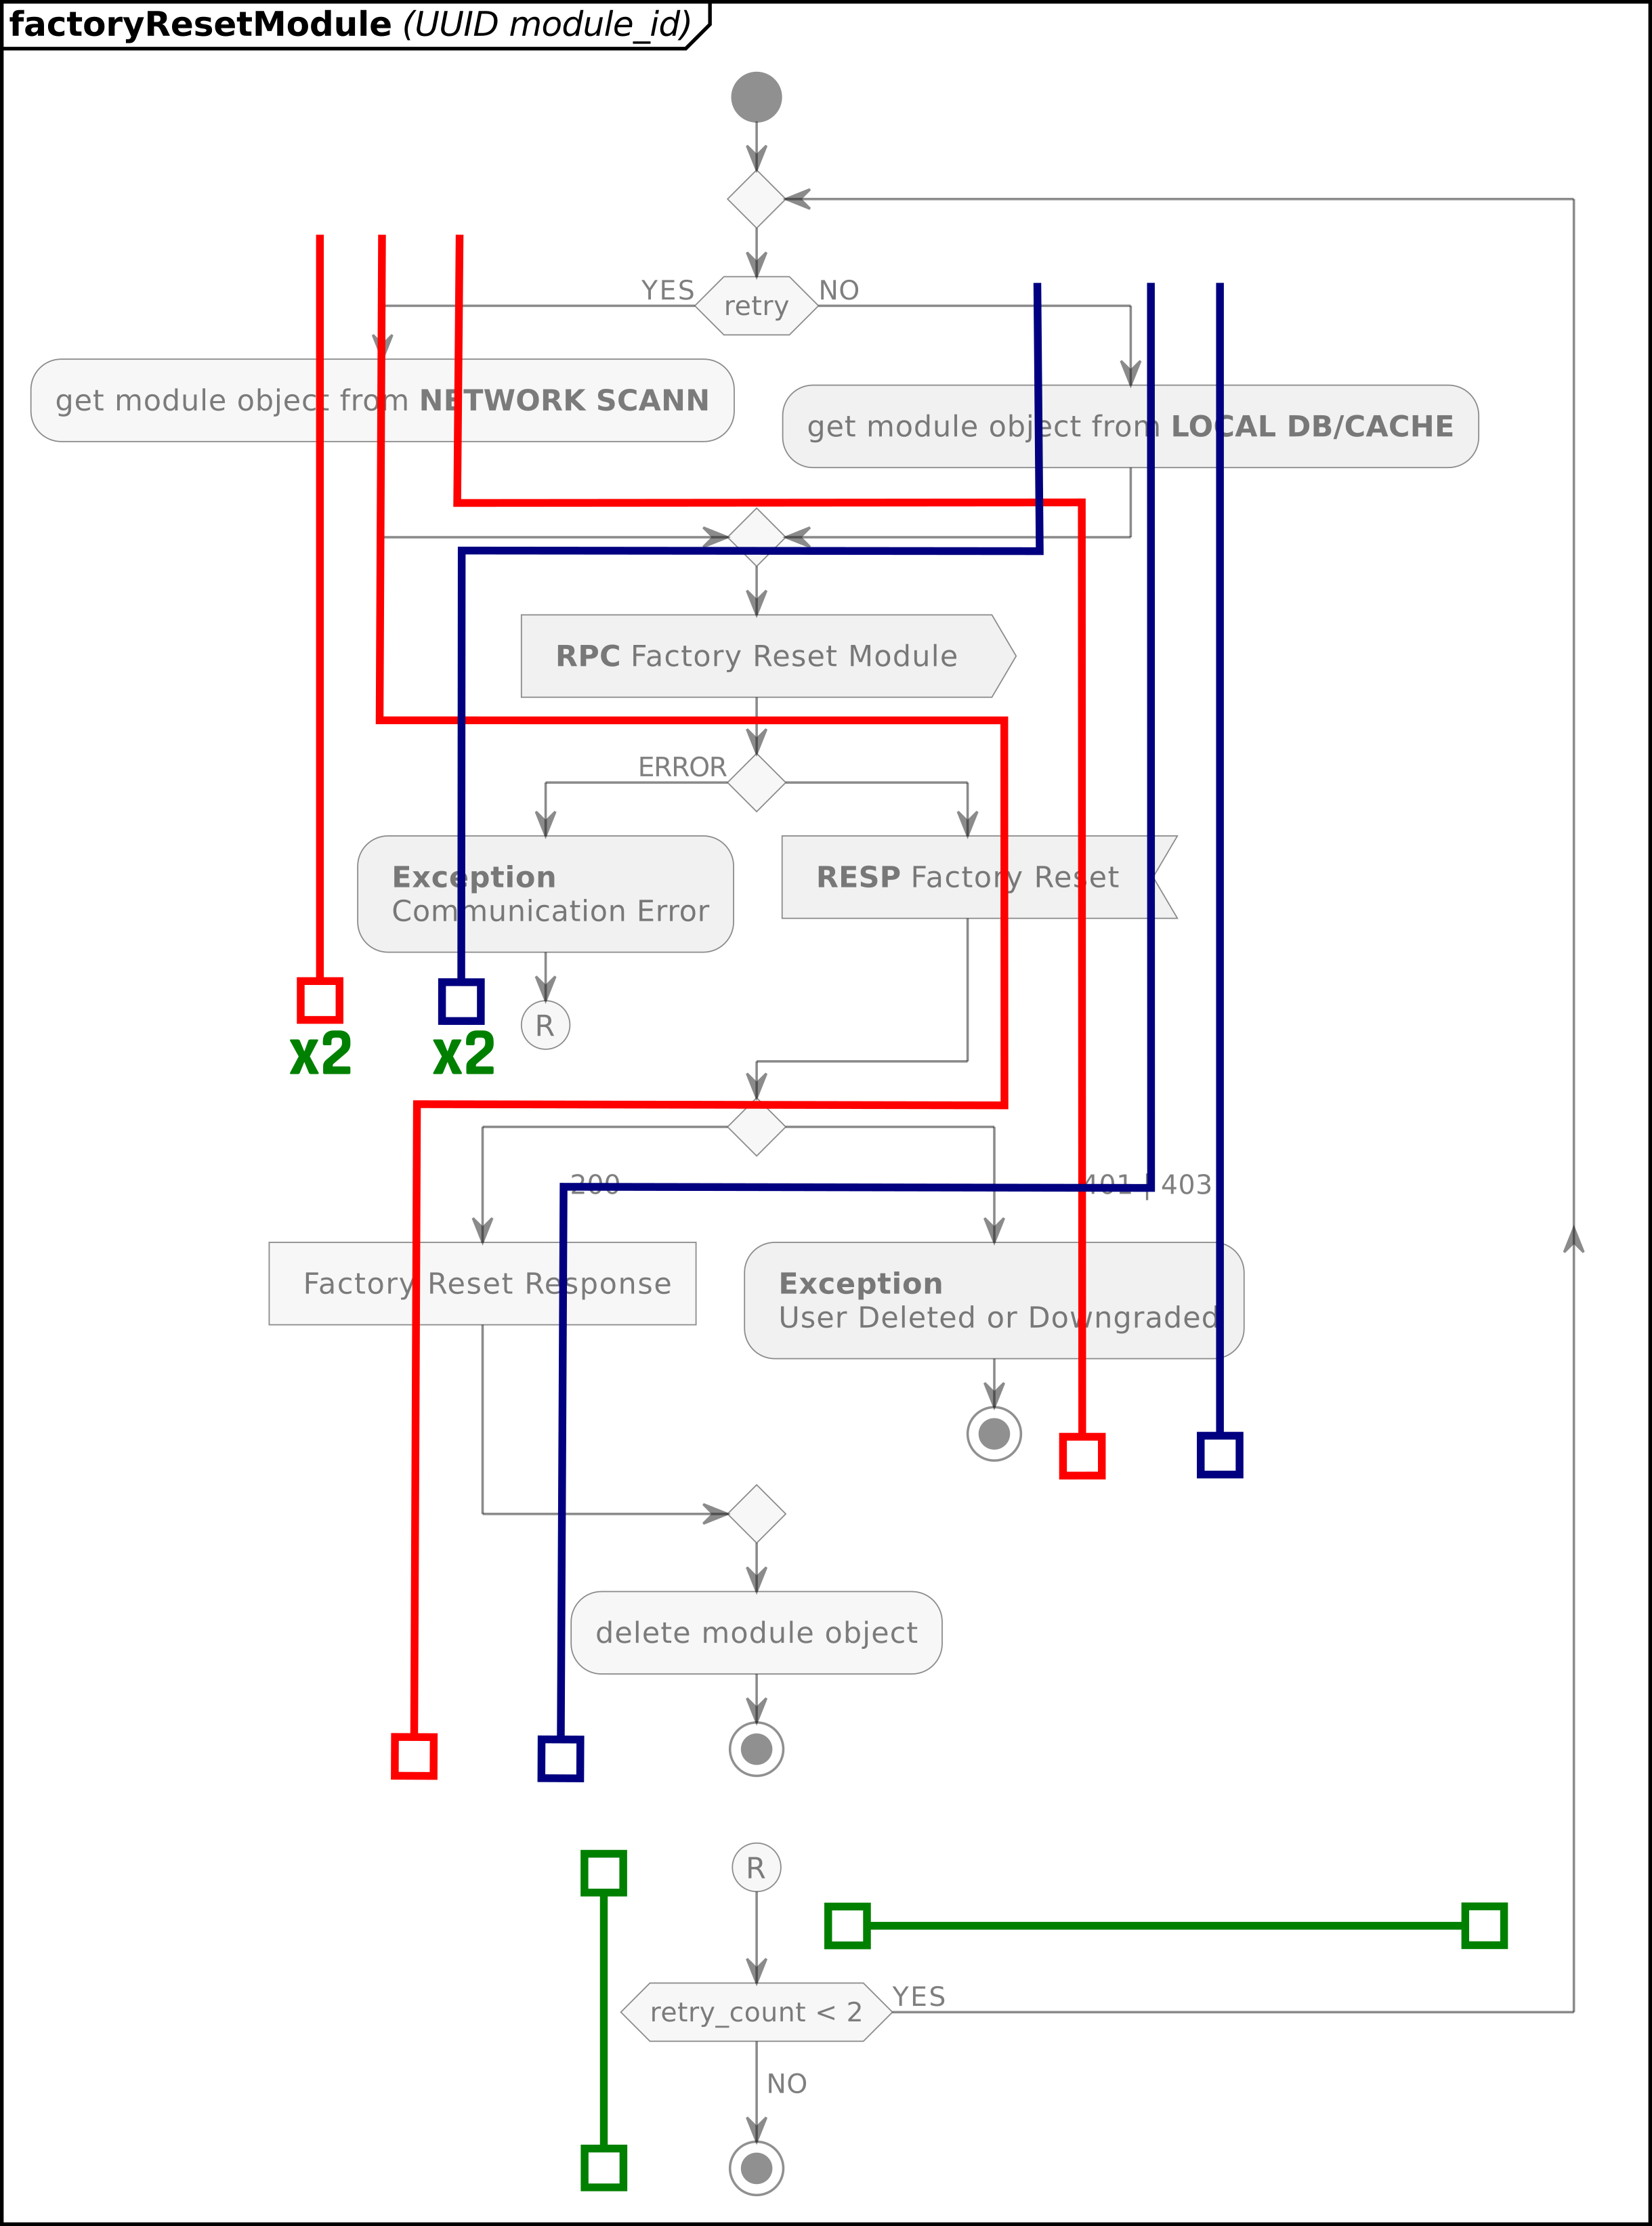
\includegraphics[width=0.8\textwidth]{Figures/iter2/ACT_factoryResetModule_branches_ink.png}
	\rule{35em}{1pt}
	\caption[Ramas sobre Caso de Uso]{Ramas de ejecución dibujadas sobre el diagrama de actividades de la implementación del caso de uso: Reinicio a Valores de Fábrica.}
	\label{fig:act_act_test_branches}
\end{figure}

En la figura ~\ref{fig:act_act_test_branches} se indican las ramas con líneas sobre el diagrama de actividades para un caso de uso. Para cada una de estas líneas se codificará un caso de prueba.

\subsection{Pruebas Unitarias}
Teniendo en cuenta la criticidad de los algoritmos implementados para la capa de datos y la lógica de negocios en la capa de dominio. Se escribieron pruebas unitarias para ambas capas. En la figura ~\ref{fig:tests_ss} se muestra el reporte de ejecución de los casos de prueba. 
%Sobre un total de Se consiguió la ejecución exitosa del total de  

\begin{figure}[H]
	\centering
	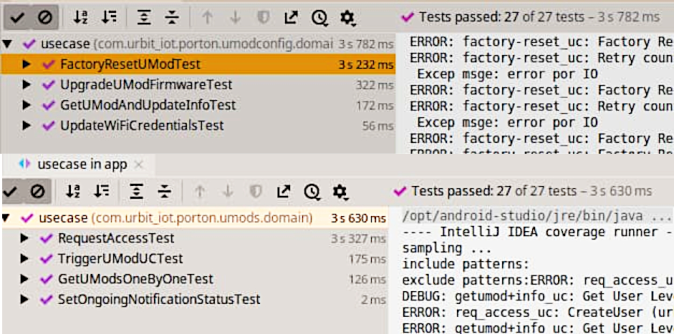
\includegraphics[width=0.6\textwidth]{Figures/iter2/tests_all.png}
	\rule{35em}{1pt}
	\caption[Captura Pruebas Unitarias]{Reporte de ejecución de pruebas unitarias en la IDE de desarrollo.}
	\label{fig:tests_ss}
\end{figure}

\subsection{Pruebas de Interfaz de Usuario}
Este tipo de prueba conocidas como ``UI Tests'' se ofrece como parte del framework Espresso de pruebas instrumentadas para android y que viene soportado por defecto por la plataforma de desarrollo. Permiten ejecutar casos de prueba sobre la aplicación real ejecutada sobre un dispositivo real sobre el cual se simulan las interacciones del usuario con la interfaz gráfica, es decir se emulan los efectos de los gestos humanos sobre la pantalla de un teléfono.
Para ello es necesario que el dispositivo en cuestión, el teléfono, esté conectado por cable USB a la computadora del desarrollador. Cuando se ejecutan las pruebas se procede con una instalación nueva de la aplicación en el dispositivo, se abre dicha aplicación y finalmente se ejecutan los casos de prueba programados usando Espresso.

Para el presente proyecto se codificaron, como demostración conceptual, solo unos casos de prueba para la pantalla principal de la aplicación, el listado de módulos. El esfuerzo se realizó con el ánimo de dejar una base sólida para mejorar el nivel de validación del desarrollo del software.\\
La puesta a punto de las dependencias y la configuración de los parámetros para conseguir ejecutar este tipo de pruebas de manera correcta se convirtió en un desafío que tomó semanas en ser resuelto mayormente debido a que se utilizó inyección de dependencias en todo el proyecto empleando Dagger.\\
%Todos los casos se ejecutaron de manera exitosa y el reporte se puede observar en la figura ~\ref{}.
Como una nota relevante para el lector que desee ejecutar las pruebas sobre un dispositivo android se le recomienda enfáticamente desactivar las animaciones en las configuraciones avanzadas de programador en dicho dispositivo.




